\chapter{Final Results and Conclusions}\label{sec:results}

In this analysis we measured the branching fraction of the charmless semileptonic $B$ meson decay \decayb~on a data sample corresponding to $710\e{fb^{-1}}$ of integrated luminosity. We present the final result, shown in chapter \ref{sec:extraction-of-physical-parameters}, with the statistical and systematic uncertainties determined in chapter \ref{sec:systematic-uncertainty}.

\section{Signal Significance}

In order to determine the signal significance, the profile likelihood function is obtained by performing the signal fit to data with a fixed signal yield. The yield is fixed to values in the range $[0, 1000]$ and, for each fit, the maximum likelihood of the fit is extracted. The signal yield at the maximum of the profile likelihood corresponds to the optimal fit value. In order to incorporate systematic uncertainties in the profile likelihood, the latter is convoluted with a Gaussian function. The width of the Gaussian function used in the convolution corresponds to the systematic uncertainty of the signal yield, meaning that only contributions that affect the signal yield are taken into account. The total systematic uncertainty on the signal yield is
\begin{equation}
\sigma_{\mathrm{sys}}^{\mathrm{yield}} = {}_{-71}^{+85}.
\end{equation}
The asymmetric systematic error is taken into account by using the negative error in the convolution for the left side of the profile likelihood, and the positive error for the right side. Figure \ref{fig:significance} (left) shows the profile likelihood as a function of the signal yield before and after incorporating systematic uncertainties, while Figure \ref{fig:significance} (right) shows the negative-log-likelihood of the profile likelihood, which is more commonly used. As mentioned in Eq. (\ref{eq:lr} -- \ref{eq:ss}), signal significance is calculated as the square-root value of $\sqrt{-2\log(\mathcal{L}/\mathcal{L}_{\mathrm{max}})}$ at the $0$ expected signal yield. In this measurement, the statistical significance of the signal yield is equal to about $6.3\sigma$, while the total significance amounts to about $4.6\sigma$.

\begin{figure}[H]
	\centering
	\captionsetup{width=0.8\linewidth}
	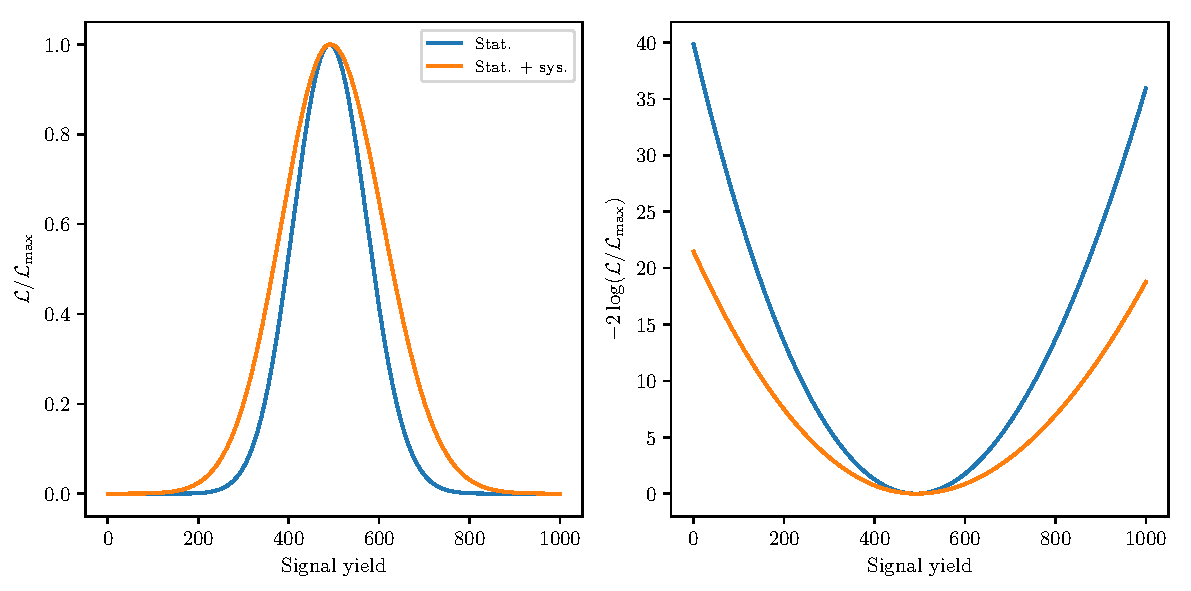
\includegraphics[width=\linewidth]{fig/significance}
	\caption{Profile likelihood function (left) and negative-log-likelihood (right) for the case with statistical error only (blue) and convoluted with a Gaussian function in order to incorporate the systematic uncertainty on the yield (orange).}
	\label{fig:significance}
\end{figure}


\section{Branching Fraction}

This work presents the first measurement of the \decayb~decay. Including the total systematic uncertainties from Table \ref{tab:sys_summary}, the final result of the signal branching ratio is
\begin{equation}
\mathcal{B}(B^+ \to K^+ K^- \ell^+ \nu) = (3.04 \pm 0.51 \pm {}^{+0.67}_{-0.66})\E{-5},
\end{equation}
where the first and the second uncertainty are statistical and systematic, respectively. With a signal significance of $4.6\sigma$, this measurement represents the first evidence for the \decayb~decay.

